\documentclass[border=6pt]{standalone}
\usepackage{tikz}
\usepackage[edges]{forest}
\usetikzlibrary{arrows.meta,positioning,calc,decorations.pathreplacing,shapes.geometric}
\begin{document}
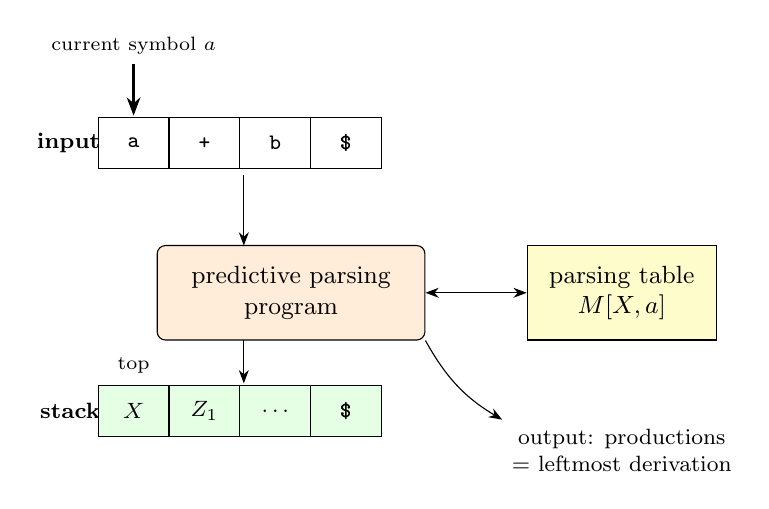
\begin{tikzpicture}[>=Stealth,font=\small,
 cell/.style={draw,minimum height=0.65cm,minimum width=0.9cm,align=center,font=\footnotesize}]
\node[font=\footnotesize\bfseries,anchor=east] at (-0.3,1.9) {input};
\foreach \i/\c in {0/a,1/+,2/b,3/\$} \node[cell] at (\i*0.9,1.9) {\texttt{\c}};
\draw[->,thick] (0.0,2.9) node[above,font=\scriptsize]{current symbol $a$} -- (0.0,2.25);
\node[draw,rounded corners=3pt,fill=orange!15,minimum width=3.4cm,minimum height=1.2cm,align=center] (pp) at (2.0,0) {predictive parsing\\program};
\draw[->] (1.4,1.5) -- (1.4,0.6);
\node[font=\footnotesize\bfseries,anchor=east] at (-0.3,-1.5) {stack};
\node[cell,fill=green!10] (x) at (0.0,-1.5) {$X$}; \node[cell,fill=green!10] (z1) at (0.9,-1.5) {$Z_1$}; \node[cell,fill=green!10] at (1.8,-1.5) {$\ldots$}; \node[cell,fill=green!10] at (2.7,-1.5) {\texttt{\$}};
\node[font=\scriptsize,anchor=south] at (0.0,-1.15) {top};
\draw[->] (1.4,-0.6) -- (1.4,-1.15);
\node[draw,fill=yellow!20,minimum width=2.4cm,minimum height=1.2cm,align=center] (tab) at (6.2,0) {parsing table\\$M[X, a]$};
\draw[<->] (pp) -- (tab);
\node[font=\footnotesize,align=center] (out) at (6.2,-2.0) {output: productions\\= leftmost derivation};
\draw[->] (pp.south east) to[bend right=15] (out.north west);
\end{tikzpicture}
\end{document}
